%************************************************
\chapter[Risk-taking behavior, urbanization and POLS]{Risk-taking behavior,
urbanization and the pace of life in birds}\label{ch:POLS}
%************************************************

% \tikz[remember picture,overlay] \node[opacity=0.3,inner sep=0pt] at (current page.center){\includegraphics[width=\paperwidth,height=\paperheight]{./Figures/cover/barco_oceano.png}};
%\tikz[remember picture,overlay] \node[opacity=0.3,inner sep=0pt] at ([yshift=6cm]current page.center){\includegraphics[width=\paperwidth,height=\paperheight]{./Figures/cover/barco_oceano.png}};
% \clearpage

\section*{Abstract}

Despite growing appreciation of the importance of considering a pace-of-life syndrome (POLS) perspective to understand how
animals interact with their environment, studies relating behavior to life history under altered environmental conditions are still
rare. By means of a comparative analysis of flight initiation distances (i.e., the distance at which an animal takes flight when a
human being is approaching) across \textgreater{300} bird species distributed worldwide, we document here the existence of a POLS
predicted by theory where slow-lived species tend to be more risk-averse than fast-lived species. This syndrome largely emerges
from the influence of body mass, and is highly dependent on the environmental context. Accordingly, the POLS structure
vanishes in urbanized environments due to slow-lived species adjusting their flight distances based on the perception of risk.
While it is unclear whether changes in POLS reflect plastic and/or evolutionary adjustments, our findings highlight the need to
integrate behavior into life history theory to fully understand how animals tolerate human-induced environmental changes.


\section*{Significance statement}

Animals can often respond to changing environmental conditions by adjusting their behavior. However, the degree to which
different species can modify their behavior depends on their life history strategy and on the environmental context. 
Species-specific perception of risk is a conspicuous example of adjustable behavior tightly associated with life history strategy. While
there is a general tendency of higher risk aversion in rural than city-dwelling birds, it is dependent on the species’ life history
strategy. Slow-lived species are more prone to adjust their flight initiation distances based on the perception of risk, allowing
humans to approach closer in urban than rural environments. Behavior must therefore be taken into account together with life
history to reliably assess species’ vulnerability at the face of ongoing environmental change.


\section{Introduction}

Behavior is widely considered one of the main mechanisms
through which animals cope with changes in the environment
\citep{Bogert1949, klopfer1962, mayr1965}. Unlike other phenotypic
features, behavior can often be rapidly modified to solve
new ecological problems, thus contributing to reduce the uncertainties
and adaptive mismatches that arise when environmental 
conditions change \citep{Huey2003, Price2003, Estrada2016, Sol2016}. 
A growing number
of studies has for instance documented that animals living
in urban environments differ in behaviors related to resource
use, disturbance avoidance, and communication from those
inhabiting little urbanized environments (reviewed in 
\citet{Shochat2006, Evans2012, Lowry2013, Sol2013a}). 
Evidence is also accumulating that these behavioral differences
primarily reflect plastic adjustments, although some
may also result either from selection or from a non-random
sorting of individuals by behaviors that affect colonization success
(reviewed in \citet{Sol2013a}).

Despite the plastic nature of most behaviors, some animals
exhibit strong consistencies in how they behave across time
and contexts (reviewed in \cite{Sih2004, Reale2007}).
These behavioral consistencies are expressed among individuals
within species, as well as among individuals of distinct
species (e.g., \citet{Moller1994, Verbeek1994, Koolhaas1999, Gosling2001, Greenberg2003, Sih2004, Reale2007}).
An example is a behavioral syndrome where
some animals are risk-averse whereas others are risk-prone
across a range of situations regardless the actual risks \citep{Sih2004, Sih2012a}.
This syndrome has attracted considerable
interest of behavioral ecologists because the inability of individuals
to adjust their behavior to the actual level of risk can
entail important costs, such as greater exposure to predators,
reduced foraging opportunities and increased energetic expenditure
\citep{Sih2004, Sih2012a}. However, the reasons why some
animals readily adjust their behavior in response to novel situations
while others persist with their behavior, even when maladaptive,
remains unresolved \citep{Sih2004}. Recently, it has
been suggested that the striking consistencies in risk-taking
behavior observed across individuals of a given species, but
not in members of other species, can be understood if we consider
behavior and life history as dimensions of a same pace-of-life
syndrome (POLS) \citep{Wolf2007, Reale2010a}.

The POLS theory argues that animals experiencing different
environmental conditions should diverge in a suite of behavioral
and physiological traits according to their life history 
\citep{Ricklefs2002, Tieleman2005, Hau2010a, Reale2010a}. 
A central premise of this theory is the existence of a
fast-slow continuum of life history variation (FS hereafter),
which reflects the impossibility to simultaneously maximize survival
and fecundity \citep{Stearns1983a, Saether1988}. The FS aligns
organisms along a pace-of-life (POL) axis from a ``highly
reproductive'' (fast-lived) strategy at one end to a ``survival''
(slow-lived) strategy at the other end. As slow-lived animals
prioritize future over current reproduction \cite{Stearns2000}, they
should generally be more risk-averse compared to those at the
fast extreme \citep{Martin2000, Wolf2007, Hau2010a, Moller2012, Moller2013a}.
In contrast, fast-lived animals should prioritize behaviors that
enhance current reproductive effort, even when doing so involves
taking some risks. Therefore, the POLS theory explicitly verbalizes
the classic idea that selection should favor behaviors ensuring
higher adult survival in slow-lived animals and behaviors that
enhance reproductive effort in fast-lived animals.

Despite the existence of theoretical predictions, empirical
support for the existence of a risk-taking POLS is currently
scarce \citep{Hille2015, Charmantier2017}. A %Wrong year for Hille 2014 in the original article
number of factors may indeed prevent the detection of such a
POLS. One is the extent to which risk-taking behaviors can be
modified by learning. Slow-lived species have less cognitive
and time constrains to gather new environmental information
and accommodate their behavior accordingly by means of
learning \citep{VanSchaik2003, Sol2009a, Sih2012, Sol2016a}.
If plastically modifying FID
depends on the position of the animal in the fast-slow continuum,
the POLS may vanish in contexts where the perception
of risk is low.

Another factor that makes the demonstration of POLS challenging
is the low heritability of life history traits \citep{Price1991}.
The analysis of individual variation within
populations is fundamental to disentangle the importance of
plasticity and genetic processes, as well as being of interest in
itself \citep{Reale2007}. However, the low heritability of life
history traits reduces the likelihood of detecting POLS at the
individual level. An obvious alternative is to examine POLS
across populations or species, as they have had more opportunities
to diverge in behavioral and life history traits, yet such
a level of analysis is more rarely used.

Here, we investigate if risk-taking behaviors are a defining
part of a POLS syndrome in birds, and ask to what extent the
syndrome can be relaxed according to the environmental conditions.
We focus on behavioral and life history differences
across species exposed to contrasting degrees of human disturbances.
Our measure of risk-taking behavior is the flight
initiation distance (FID), defined as the distance at which an
individual takes flight when approached by a human. Previous
work in birds has shown that FID within and across species is
shorter in urbanized than in non-urbanized environments
\citep{Moller2008, Carrete2011, Sol2012b},
indicating that the perception of risk is context-dependent. We
take advantage of these previous findings to address two main
expectations of POLS theory regarding risk-taking behavior.
The first is the expectation that slow-lived species should exhibit
longer FID than fast-lived species when the perception of
risk is high. Although FID has been found to be positively
related to certain vital rates in birds, like fecundity \citep{Blumstein2006, Moller2012}, 
the fast-slow continuum
is better characterized in the context of the full life cycle of a
species \citep{Adler2014}. We operationally defined the continuum
as the combination of life history traits that better
predicts the fecundity-survival trade-off \citep{Caswell2000, Oli2003, Oli2004}. 
We then used information on
\textgreater{11,000} measures of FID belonging to \textgreater{300} avian species to
ask whether flight distances vary depending on the position of
the species in the fast-slow continuum. To this purpose, we
used phylogenetic Bayesian mixed models that allow the integration
of species-level information generated by observations
of multiple individuals. As theoretical and empirical evidence
suggests that both the fast-slow continuum \citep{stearns1992evolution} 
and FID \citep{Moller2015} are positively correlated with
body size, we also examined whether body size may be one of
the factors underlying the FID-FS association.

The second expectation of POLS theory is that slow-lived
species can better accommodate their FID to the perception of
risk than fast-lived species. This expectation derives from the
supposed higher behavioral plasticity of slow-lived species
\citep{Sol2009}, which would allow them to habituate faster to
human presence, and from constraints in fast-lived species to
adopt risk-averse strategies due to the need to prioritize reproduction.
We validated this prediction by investigating how
FIDs change between urban and rural habitats as a function
of the position of the species in the fast-slow continuum, again
using phylogenetic Bayesian mixed models. Following suggestions
that behavioral differences between urban and non-urban
birds might be linked to brain size and learning capabilities
\citep{Kark2007, Maklakov2011, Sol2011}, 
we also verified whether a larger brain size contributes
to explain why slow-lived species should be better able to
accommodate FID to risk perception \citep{Sol2009a, Sol2009}.


\section{Material and methods}

\subsection*{Measuring FID}

A total of 11,863 FID observations were recorded by one of
the authors (APM) during February–September 2006–2014,
using a standard experimental field procedure \citep{hediger1934biologie, hemmingsen1951relation, Blumstein2006}. 
All estimates were collected
blindly with respect to the hypotheses being tested here,
thereby preventing any conscious or unconscious bias. The
observations were made in an area of 100 km2 in Orsay (48°
42’ N, 2° 11′ E, France), 800 km2 in Northern Jutland (57° 12’
N, 10° 00′ E, Denmark), 500 km2 in Oslo (59° 54’ N, 10° 45′
E, Norway), and 500 km2 on Hainan Island (19° 12’ N, 109°
42′ E, Southern China). In most regions, observations were
carried out in both urban habitats (i.e., areas with multistory
buildings, single-family houses, roads, and urban parks) and
rural habitats (i.e., open farmland and woodland lacking continuous
urbanized areas). Therefore, our distinction between
urban and rural habitats essentially separates environments
very frequented by humans from those less frequented.

To record FIDs, the observer located an individual bird
with binoculars and subsequently moved at a normal walking
speed towards the individual, while counting the number of
steps (which approximately equals the number of meters
\citep{Moller2008}). The FID was the horizontal distance at which
the individual took flight. The starting distance (i.e., the distance
from where the observer started walking up to the bird)
was in most cases (\textgreater{98\%} of all observations) fixed at ca. 30 m
to avoid confounding FID with starting distance. If the bird
was located in the vegetation, the height above ground was
also recorded to the nearest meter using the observer as a
yardstick. This method is reliable when cross-validated using
a laser Bushnell® Elite 1500. FID was then estimated as the
Euclidean distance, which equals the square-root of the sum of
the squared horizontal distance and the squared height above
ground level \citep{Blumstein2006}. When possible, sex (n = 4958
observations), age (n = 10,887), and flock size (n = 1387)
were also recorded to be included as confounds in the models.
Although the FID of some individuals was measured twice,
we only used the first measure in the analyses. All FID data
are available as supplementary material.


\subsection*{Measuring POL}

To estimate the fast-slow continuum, we searched for published
information on six life history traits: (1) clutch size,
(2) number of broods per year, (3) maximum lifespan (years),
(4) incubation period (days), (5) nestling period (days), and
(6) age at first reproduction (years). We found information of
all six traits for 765 avian species (see \citet{Sol2016a}). As
originally defined, the fast-slow continuum results from the
existence of a fecundity-survival trade-off \citep{stearns1992evolution}.
Consequently, we empirically defined the fast-slow continuum
as the combination of life history traits that better predicts
the relative sensitivity (i.e., elasticity) of population growth to
changes in adult survival \citep{Caswell2000, Oli2003, Oli2004}. 
To this purpose, we used the COMADRE
Matrix database \citep{Salguero-Gomez2016} to obtain 
age-structured population matrices that incorporate accurate information
on the rates of survival, growth, and reproduction from
natural populations. We removed four matrices for which elasticities
did not sum up to 1, which could reflect mistakes in the
data, and for the remaining matrices (n = 53 from 49 species),
we estimated the elasticity for adult survival. To combine the
life history traits, we conducted phylogenetic principal
component analyses (PPCA) \citep{Revell2009a} based on the 765
species, including a minimum of three traits in each analysis
(i.e., 42 PPCAs). The species scores of each PPCA was then
used as predictor of elasticities in a phylogenetic least square
models (PGLS) \citep{Orme2013}, and the best models were
classified according to AICc. The combination of life history
traits that best predicted variation in elasticity for adult survival
included lifespan, clutch size, and fledging period. We
therefore defined the position of each species in the fast-slow
continuum by extracting the scores of this PPCA. In
our best PPCA, species with high scores (i.e., high adult survival
elasticities) were slow-lived and those with low scores
(i.e., high fecundity elasticities) were fast-lived. We note that
the results of our approach based on adult survival elasticities
are similar to those based on estimates of elasticities for fecundity
or on generation time extracted from the demographic
matrices (see Chapter \ref{ch:LHaxes}).


\subsection*{Modeling FID}

To model variation in FID, we used Bayesian phylogenetic
mixed models (BPMM) with Gaussian error structure, as im-
plemented in the R package ``MCMCglmm'' \citep{Hadfield2010, Hadfield2010a}. 
FID was log transformed before
analyses to improve model convergence. As our units of
analysis were the FID observations, species identity was included
as a random factor together with phylogeny. The phylogeny
was a maximum clade credibility phylogeny (CCP)
consensus tree based on a sample of 1000 phylogenies from
the pseudo-posterior distribution in \citet{Jetz2012}, built with
the TREEANNOTATOR software \citep{Drummond2012}.
When appropriate, country was also included as a random factor
to better account for data heterogeneity (see results for details).
We first ran models without predictors to estimate FID
consistency within species and phylogenetic heritability by
means of a variance components analysis \citep{Housworth2004}. 
Then, we added predictors as fixed effects to explain
variation in FID. To demonstrate the existence of POLS, we
modeled FID as a function of the fast-slow continuum, including
habitat (i.e., rural or urban), sex, age, flock size, and height
at which the bird was observed as possible confounding effects.
Using non-informative priors, the MCMC chains were run for
330,000 iterations with a burn-in interval of 30,000 and sampling
each 300 iterations to ensure satisfactory convergence.

As we found evidence for a link between FID and FS, we
tested whether this was caused by their common association
with body size. To this purpose, we used phylogenetic path
analyses on species’ trait averages \citep{VonHardenberg2013, Gonzalez-Voyer2014}. 
The minimal set of conditional independencies for each
path model \citep{VonHardenberg2013} was
tested using PGLSs models as implemented in the package ape
\citep{Paradis2004} in R. Models were run estimating an evolutionary
parameter ($\lambda$) simultaneously with model fit that adjusts
the variance–covariance matrix to adequately fit the model
of evolution, in our case a Brownian motion model \citep{Freckleton2002}. 
The fit of a given path model to the data was
estimated via the C statistic. The C statistic tests whether the
minimum set of conditional independencies of a model is fulfilled
by the observational data, thus it provides an estimate of
the goodness of fit of the model to the data \citep{Shipley2013}. A
significant C statistic indicates that the model is a poor fit to the
data. We employed an information theoretical approach and
compared the different path models using the C statistic information
criterion (CICc; analogous to the Akaike information
criterion; \citet{VonHardenberg2013}).

We finally investigated whether changes in FID between
urban and rural habitat were larger in slow-lived species than
in fast-lived species, using the same BPMM approach described
above. To do so, we averaged the FID values of each
species per habitat and then estimated FID difference as
$$log(mean FID_{rural}) - log(mean FID_{urban})$$
We therefore only
used species present in both habitats for the analyses. FID
differences were then used as response variable in a BPMM
with the fast-slow continuum as fixed effect and the phylogeny
as a random factor. Unlike previous models, the level of
analysis here was the species instead of FID observations.
Thus, the conclusions could be sensitive to the sample size
used to estimate FID differences. We tackled this limitation in
two ways. First, in the BPMM we weighted FID differences
by 1/(n−3), being n the number of individuals sampled per
species. Second, we re-ran the model for the subset of species
with at least 15 FID observations in each habitat. To test
whether differences in FID across habitats were related to
differences in brain size, we used information published in
\citet{Sayol2016} on the residuals of a log-log PGLS of brain
volume against body mass. Positive residuals mean that the
brain of the species is larger than expected by body size and
negative residuals that is smaller than expected by body size.


\section{Results}

\begin{figure}
\centering
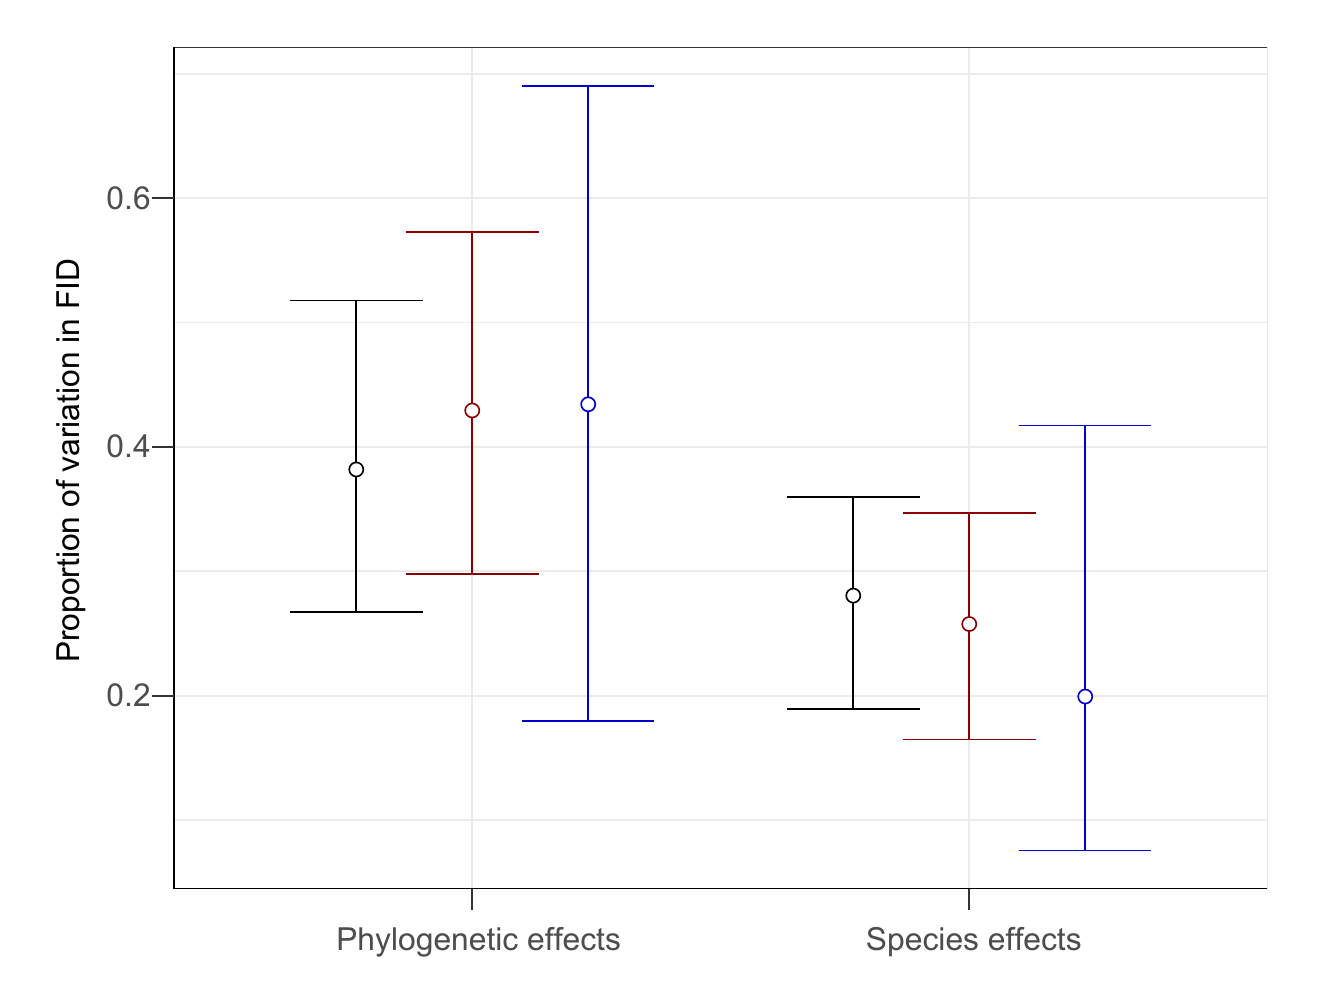
\includegraphics[width=0.75\textwidth]{./Figures/chapter04/Fig_1.png}
\caption[Variance in FID accounted for the phylogeny and species]{
Proportion of variance in FID accounted for the phylogeny and
within species variation when considering all observations (black), rural
observations only (red) and urban observations only (blue). Values are the
intra-class coefficients estimated by means of a BPMM with the constant
as fixed effect and the phylogeny and species identity as random factors.
Error bars are 95\% credible intervals.}\label{fig:fig4.1}
\end{figure}

A Bayesian phylogenetic mixed model (BPMM) based on 11,852
observations of 317 bird species confirmed the existence of consistent
among-species variation in FID (mode = 0.65, CI = 0.57–
0.77), much of which was shared among close relatives (Fig. \ref{fig:fig4.1},
Table \ref{tab:tabApp4.1}). FID did not vary with sex (pMCMC = 0.920), age
(pMCMC = 0.518), and flock size (pMCMC = 0.696). However,
birds did tend to exhibit longer FID when located at certain height
above the ground (mode = 0.026, CI = 0.013–0.038). Of the remaining
residual variation, a significant fraction was accounted for
differences among habitats. As shown in previous studies
(reviewed in \citet{Moller2014a}), FID was consistently shorter in urban
than in rural habitats across all study regions (pMCMC \textless{0.0001},
Fig. \ref{fig:fig4.2}, Table \ref{tab:tabApp4.2}). Variation in FID across species was also more
consistent in rural than in urban habitats (Fig. \ref{fig:fig4.1}).

\begin{figure}
\centering
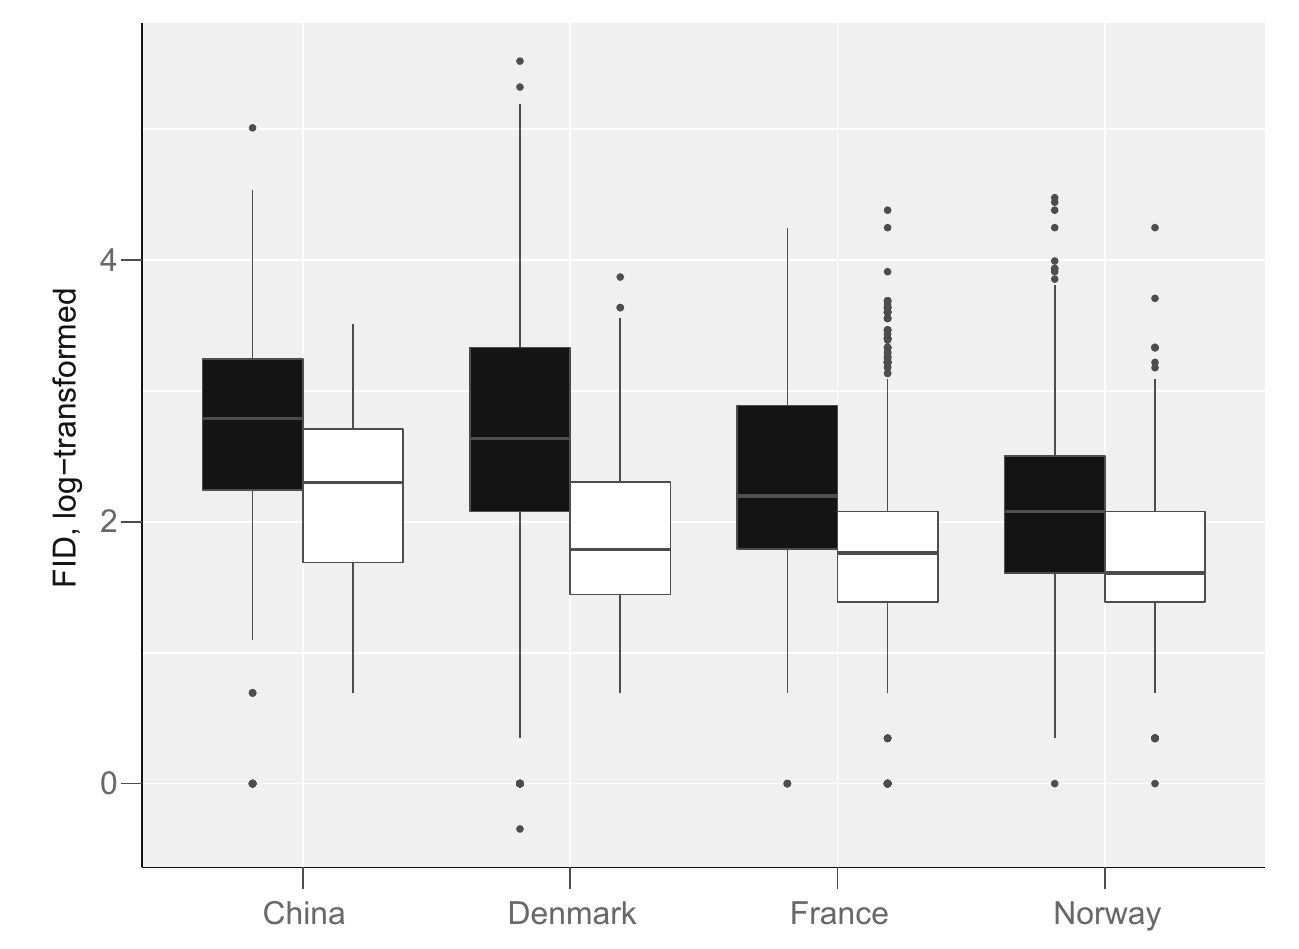
\includegraphics[width=0.75\textwidth]{./Figures/chapter04/Fig_2.png}
\caption[FID across countries]{Differences in FID between urban (white) and rural
(black) habitats across countries. The plot shows the median,
interquantile range and 1st and 3rd quartiles.}\label{fig:fig4.2}
\end{figure}

The studied species exhibited substantial variation in their
position along the fast-slow continuum, reflecting the existence
of a fecundity-survival trade-off (Fig. \ref{fig:fig4.3}). As expected, species at
the slow extreme of the continuum tended to exhibit longer FID
than those at the fast extreme (pMCMC \textless{0.0001}, Table \ref{tab:tabApp4.3}),
consistent with the existence of a POLS. However, there was a
negative interaction with habitat (Table \ref{tab:table4.1}), reflecting that FID
and life history variation became decoupled in urban environments
(Fig. \ref{fig:fig4.4}). This pattern was largely due to changes in FID
across habitats by slow-lived species (Table \ref{tab:table4.2}, Fig. \ref{fig:fig4.4}). In rural
environments, where the POLS was detected, the best phylogenetic
path models suggest that the FID-FS association was primarily
caused by their common association with body size
(Figs. \ref{fig:fig4.5}, \ref{fig:figApp4.2}). In urban environments, there is no direct effect of
body size on FID, which might explain why the FID-FS association 
is no longer present (Figs. \ref{fig:fig4.5}, \ref{fig:figApp4.3}).

\begin{figure}
\centering
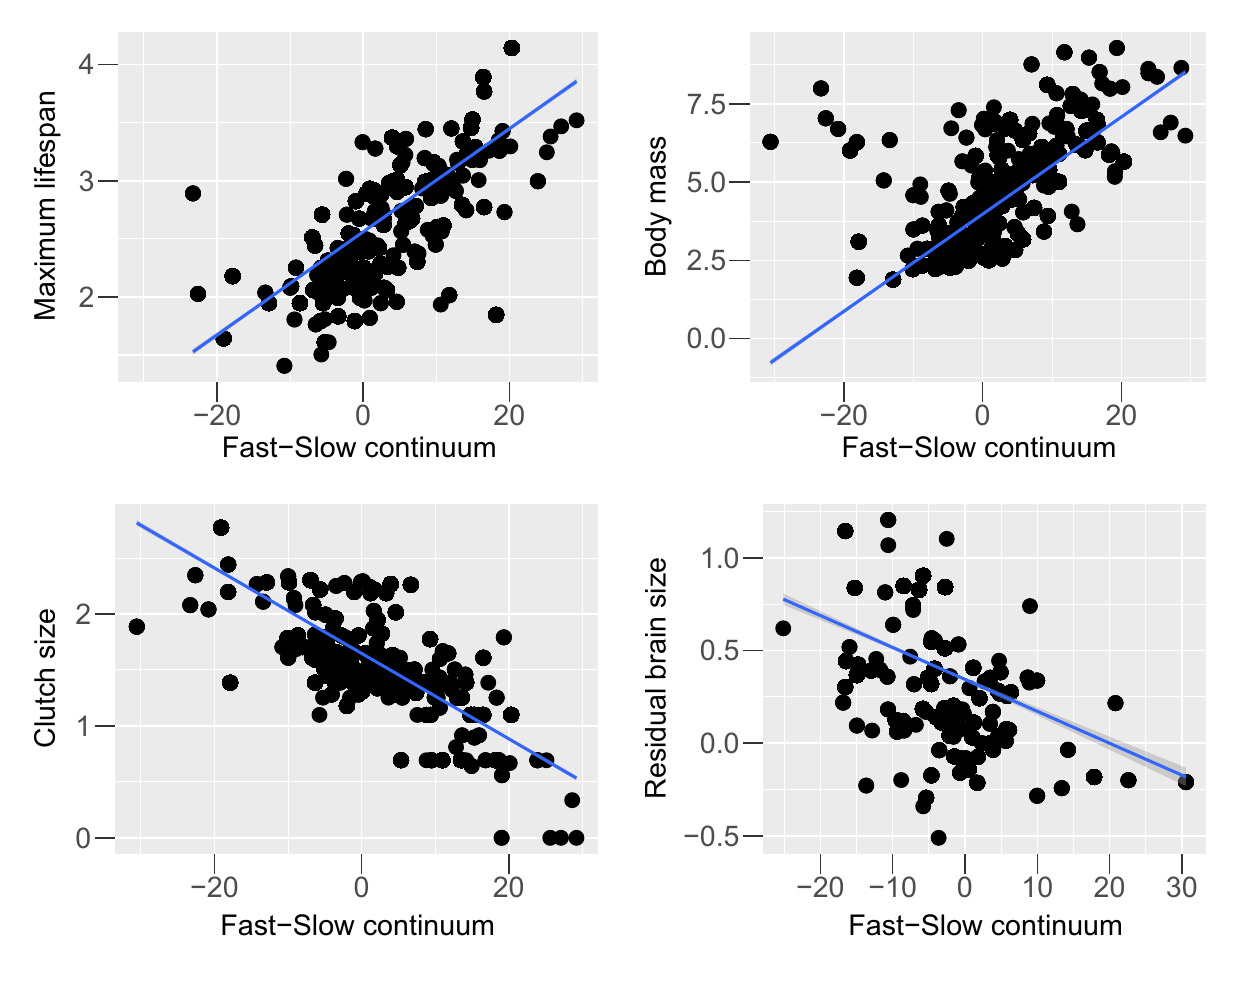
\includegraphics[width=\textwidth]{./Figures/chapter04/Fig_3.png}
\caption[Fast-slow continuum and LH traits]{Relationship of the fast-slow continuum (FS) across species with maximum lifespan,
clutch size, body mass, and residual brain size. The three first
traits have been log transformed. Residual brain size represent the
residuals of a log-log PGLS of brain volume against body mass
(i.e., positive residuals mean that the brain of the species is larger
than expected by body size and negative residuals that is smaller
than expected by body size).}\label{fig:fig4.3}
\end{figure}

Because slow-lived species tend to have disproportionally
larger brains than fast-lived species (Fig. \ref{fig:fig4.3}), the reduction in
FID observed in slow-lived species could reflect enhanced learning 
capacities. Species with larger brain residual exhibited longer
FID in rural habitats than those with smaller brain residual
(pMCMC = 0.008, Table S4), but they did not experience a more
substantial change in FID between rural and urban habitats
(Table \ref{tab:tabApp4.5}).


\begin{table}
\caption[Best model for FID]{BPMM accounting for variation in FID (response
variable, log transformed) as a function of the interaction
between habitat and the fast-slow continuum, based on information
from all regions for which both urban and rural FID observations
were available (Denmark, France, Norway, and China). The model
was run with a Gaussian structure of the errors and a non-informative
prior, the number of iterations being defined by nitt = 330,000,
burnin = 30,000 and thin = 300.}\label{tab:table4.1}
\begin{tabular}{llllll}
\toprule
            & \textbf{post mean} & \textbf{L-95\% CI} & \textbf{U-95\%} & \textbf{eff.samp} & \textbf{pMCMC} \\
\multicolumn{6}{@{}l@{}}{\textbf{Random effects}}                                       \\
Phylogeny        &               &               &        &          & -                \\ % TODO: missing values
Species          & 0.143         & 0.095         & 0.199  & 1000     & -                \\
Country          & 0.168         & 0.011         & 0.477  & 1000     & -                \\
Residual         & 0.196         & 0.190         & 0.201  & 1000     & -                \\
\multicolumn{6}{@{}l@{}}{\textbf{Fixed effects}}                                        \\
Intercept        & 3.123         & 2.567         & 3.669  & 1000     & \textless{0.001} \\
FS               & 0.024         & 0.0114        & 0.035  & 1000     & \textless{0.001} \\
Habitat:urban    & -0.321        & -0.3444       & -0.299 & 1000     & \textless{0.001} \\
Height           & 0.014         & 0.0114        & 0.017  & 1000     & \textless{0.001} \\
FS*Habitat:urban & -0.032        & -0.035        & -0.028 & 1000     & \textless{0.001} \\
\bottomrule
\end{tabular}
\end{table}


\section{Discussion}

\begin{figure}
\centering
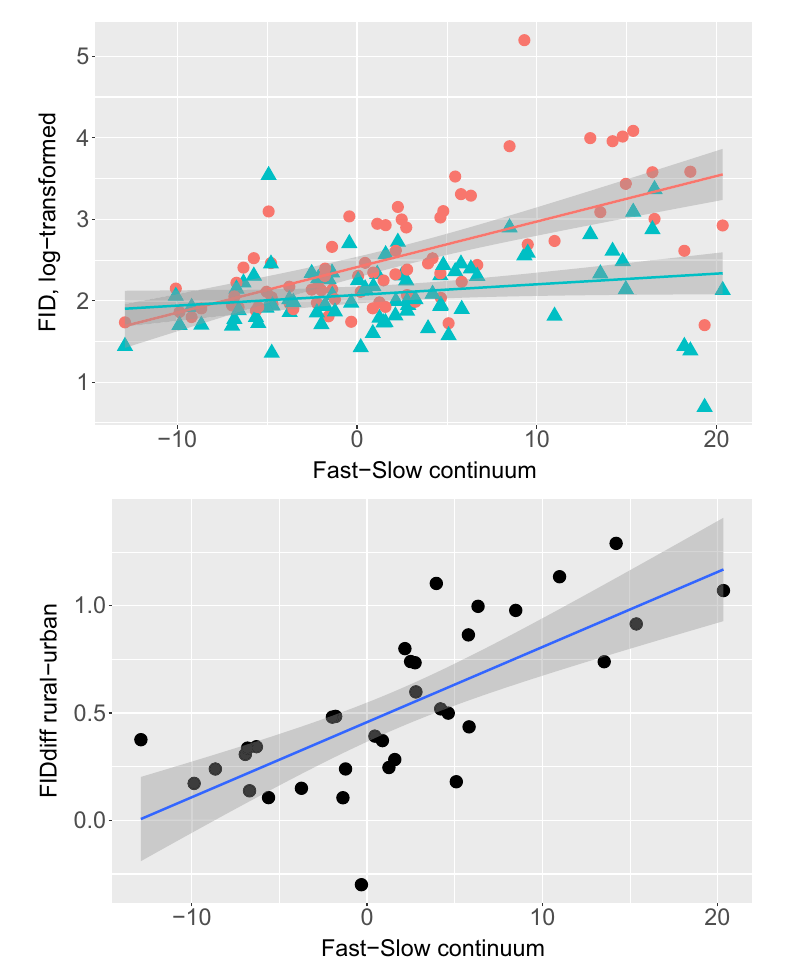
\includegraphics[width=.75\textwidth]{./Figures/chapter04/Fig_4.png}
\caption[FID and fast-slow continuum]{Above, relationship between FID and the fast-slow continuum for
urban (blue triangles) and rural (red circles) habitats. Below, difference in
FID between rural and urban habitats as a function of the fast-slow continuum.}\label{fig:fig4.4}
\end{figure}


\begin{table}
\caption[Best model for rural and urband differences in FID]{BPMM accounting for the decline in FID per species from
rural and urban habitats (response variable) a function of the fast-slow
continuum, based on information from species for which both urban and
rural FID observations were available. The decline of each species was
estimated as the $log(mean FID_{rural}) - log(mean FID_{urban})$. The model was
repeated again restricting the species to those with at least 15 FID
observations in each habitat. The models were run with a Gaussian structure
of the errors and non-informative priors. We weighted the observations
by $1/(n-3)$, being ``$n$'' the number of FID observations of the species.
The model was run with a Gaussian structure of the errors and a
non-informative prior, the number of iterations being defined by nitt =
440,000, burni = 40,000 and thin = 400.}\label{tab:table4.2}
\begin{tabular}{llllll}
\toprule
\multicolumn{6}{l}{\textbf{Model with all species}}                                                            \\
\midrule
              & \textbf{post mean} & \textbf{L-95\% CI} & \textbf{U-95\%} & \textbf{eff.samp} & \textbf{pMCMC} \\
\multicolumn{6}{@{}l@{}}{\textbf{Random effects}}                                 \\
Phylogeny             & 0.074     & 0.000     & 0.197  & 539      & -             \\
Residual              & 0.086     & 0.035     & 0.152  & 637      & -             \\
\multicolumn{6}{@{}l@{}}{\textbf{Fixed effects}}                                  \\
Intercepts         & 0.560     & 0.283     & 0.857  & 889.5    & \textless{0.001} \\
FS                 & 0.031     & 0.015     & 0.048  & 718.4    & 0.002            \\
\noalign{\bigskip}
\toprule
\multicolumn{6}{l}{\textbf{Model with  species with at least 15 FID observations per habitat}}               \\
\midrule
           & \textbf{post mean} & \textbf{L-95\% CI} & \textbf{U-95\%} & \textbf{eff.samp} & \textbf{pMCMC}  \\
\multicolumn{6}{@{}l@{}}{\textbf{Random effects}}                                 \\
Phylogeny          & 0.095     & 0.019     & 0.192  & 794      & -                \\
Residual           & 0.018     & 0.000     & 0.043  & 703.6    & -                \\
\multicolumn{6}{@{}l@{}}{\textbf{Fixed effects}}                                  \\
Intercepts         & 0.711     & 0.358     & 1.010  & 1000     & \textless{0.001} \\
FS                 & 0.021     & 0.006     & 0.036  & 878.2    & 0.006            \\
\bottomrule
\end{tabular}
\end{table}


\begin{figure}
\centering
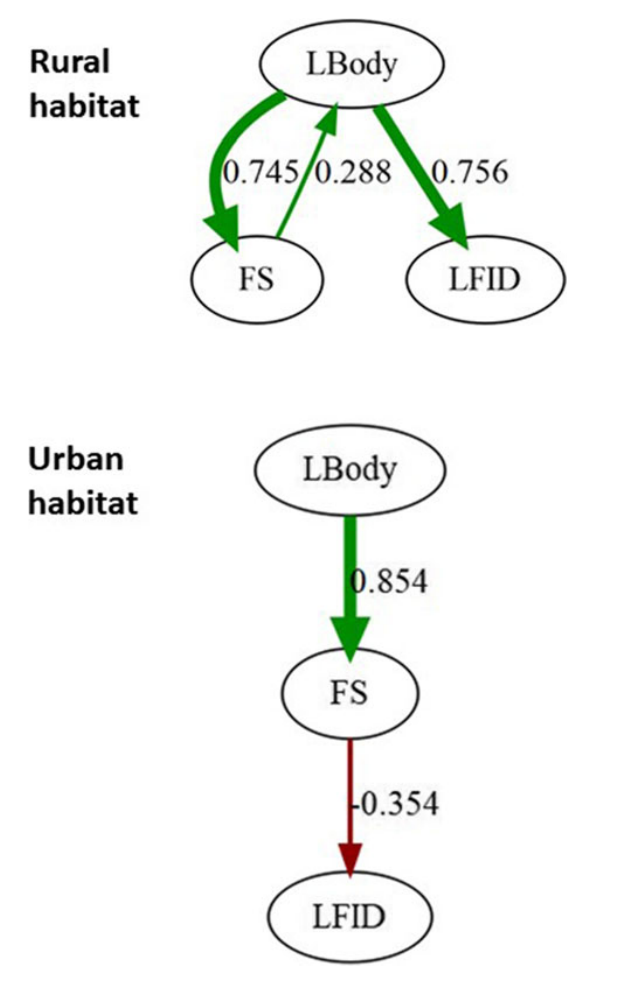
\includegraphics[width=0.5\textwidth]{./Figures/chapter04/Fig_5.png}
\caption[Phylogenetic path models for rural and urban habitats]{
Phylogenetic path model averaged over all tested models (see
Figs. S2 and S3, in the supplementary material) for rural and urban habitats,
depicting the relationship between flight initiation distance (log transformed,
LFID) and the fast-slow continuum (FS) according to differences in body mass
(LBody) across species.}\label{fig:fig4.5}
\end{figure}


Life history theory has mostly been developed under the view
that organisms are passive subjects of selection, ignoring that
behavior largely mediates how animals interact with their environment 
\citep{Sol2016}. However, recent years
have witnessed an increased appreciation that behavior can
co-vary with the life history, an idea crystalized in the POLS
concept \citep{Ricklefs2002, Reale2010a}. Our
results are in line with this new paradigm, confirming previous
suggestions and evidence that FID can be part of a POLS.

Our finding that slow-lived species tend to be more risk-averse
than fast-lived species in natural conditions fits well
with life history theory. The fitness of slow-lived animals
largely depends on ensuring a long reproductive life \citep{Stearns2000}; 
hence, individuals should favor risk-avoidance strategies
when the perception of risk is high \citep{Martin2000, Wolf2007, Hau2010a, Moller2012, Moller2013a}. 
Under this view, behavior would be a
consequence of life history. However, our analyses suggest that
the relationship between FID and the fast-slow continuum is
largely mediated by differences in body size among species.
As body size is a major determinant of the fast-slow continuum,
this does not deny the existence of a POLS. However,
larger species may also decide to flee before than smaller species
for reasons not directly induced by their life history, including
a higher likelihood to be detected by predators, lower
maneuverability to escape when attacked and higher energetic
costs associated with flight \citep{Blumstein2006}.

An animal that is unable to tolerate human presence is likely
to have problems to feed, communicate, or mate in densely
populated urban environments. This may explain why FID is
shorter in urban than in rural environments \citep{Moller2010, Moller2015a}. 
While slow-lived species showed shorter
or larger FID according to the perception of risk, fast-lived
species did not accommodate their FID to the degree of human
frequentation. The changes in FID observed in slow-lived species
may reflect plastic adjustments, selection, and/or a non-random 
sorting of individuals by behaviors that affect invasion
success. Our analyses do not allow us to distinguish between
these alternatives, although plasticity is an obvious possibility.
After detecting an approaching human, animals may decide to
ignore the threat or to flee, and cognition may be involved in
allowing informed decisions \citep{Moller2014a}. Some
animals are, for instance, able to discriminate between people
that pose a threat from people that do not \citep{Levey2009, Lee2011}. 
There is also evidence that fear of humans can
diminish when individuals are exposed to human presence for
long periods (e.g., \citet{Perals2017}). However, current
evidence that FID may be modified by habituation in the wild
remains inconclusive \citep{Moller2015}. Indeed, we did not find
evidence that enlarged brains facilitate accommodating FID to
the perception of risk, although this may simply indicate that
habituation to humans does not require the type of advanced
cognition associated with enlarged brains \citep{Overington2009}. 
Our insufficient understanding of how cognition and
neural structures affect FID is also highlighted in the fact that
we found that species with relatively larger brains exhibited
longer FID, while a previous study found the opposite pattern
\citep{Moller2014a}. As big-brained species tend to be
at the slow extreme of the fast-slow continuum, the weak effect
we found may be a mere by-product of the association between
the FID and life history. Another possibility is that sense organs
like eyes play a role in determining flight distance, with brain
size only secondarily accounting for the response \citep{Moller2014a}.

The reasons why fast-lived species did not see their FID
altered according to the perception of risk are also unclear.
While it may be argued that these species already possess
the appropriate behavior to persist in cities, it remains intriguing
why they do not increase their FID in places where interactions
with humans are rare enough to allow habituation.
Elucidating whether this reflects constrains, perhaps associated
with life history trade-offs, will represent an important avenue
for future research. The existence of substantial phylogenetic
heritability in FID, particularly when recorded in rural
habitats, is consistent with the existence of such constrains
\citep{Blomberg2003}. Further examples of possible
constrains can be found in \citet{Moller2013}, who reported that
while FID of several species of birds became shorter after a
cold winter, this was only true in resident urban populations
(frequently exposed to humans) but not in migratory or rural
populations of the same species.

Much past theoretical and empirical work on life history has
attempted to understand why organisms have diversified in a
plethora of life history strategies \citep{stearns1992evolution}. The possibility
that certain life histories offer advantages over others when it
comes to adjustment to environmental changes has also been
acknowledged (e.g., \citet{Saether2003}), but empirical
support has been more difficult to assemble (but see \citet{Sol2012a, Sol2014}). 
Similarly, little effort has focused on considering
behavior as a component of life history (e.g., \citet{Blumstein2006, Moller2012}, 
despite recent calls for the need
to integrate behavior into life history theory to better understand
how animals cope with environmental changes (reviewed in 
\citet{Sol2016}; see also \citet{Estrada2016}). Our discovery
of a POLS associated with risk-taking behavior contributes
to fill these gaps, suggesting new ways by which behavior
and life history interact to influence the response of animals to
sudden changes in their environment.

